\section{Finite precision computation}

Unfortunately for computer scientists, the world is not solely
restricted to integers, and computers often need to work with real
numbers ($\mathbb{R}$). With integers, the main problem we have in
computer terms is overflow, and since there is a finite distance from
one to the next, they are easy to encode in a computer.

On the other hand, there are infinitely many real numbers, between any
two real numbers, and since computers are discrete, we need to sample
the real numbers so that we can find a representation for them in the
computer. However, this introduces errors, since we can't represent
every value exactly (this requires an infinite number of bits) and
therefore we must approximate.

\subsection{Floating point numbers}

%Slide 1

One problem we have with computers is that we don't know what the
error is when we perform computations; how `good' is the result of an
algorithm or computation? We would like to know the error bounds of a
solution, and have the output be reliable.

%Slide 2

In the $70$'s, it was realised that different floating point
implementations produced different results. This had significant
concerns for reproducability, and as a result the ANSII IEEE standard
for binary floating point arithmetic was created.

%Slide 3

Each floating point number is represented as four integers; the base,
the precision, the exponent and the mantissa.

\[
  x = \pm m \times b^{e-n}
\]

Where:

\begin{center}
  \begin{tabular}{>{$}l<{$}|l}
    m & The mantissa (the bit before the decimal place,
        $0\leq m \leq b-1$)\\
    b & The base (or radix), usually two or ten\\
    e & The exponent (the power of the radix)\\
    n & The precision (the number of digits in the mantissa)
  \end{tabular}
\end{center}

This could alternately be written as:

\[
  x = \pm 0.d_1\dots d_n\times b^e = \pm \left(\frac{d_1}{b}
  + \dots \frac{d_n}{b_n}\right)\times b^e
\]

We say that if $d_1\neq 0$ the number is normalised (i.e. we want to
write the number as $1.0\times 10^{-2}$ rather than $0.01\times
10^1$). Using these conventions, we can normalise the way in which we
represent numbers and at least all computers will get the same errors.

% Slide 4

The amount of numbers we can represent with the floating points depends on the
values permissible for $b,n$ and $e$. When $b=2,n=2$ and $e=[-2\dots2]$:

\marginpar{The Python code used to generate this is found in the
\texttt{/COMP36212/programs} folder of the source for these notes.}

\begin{center}
\begin{tabular}{>{$}c<{$} >{$}c<{$} >{$}c<{$} >{$}c<{$} >{$}c<{$}}
1.0 & \times & 2^{-2} & = & 0.250000\\
1.1 & \times & 2^{-2} & = & 0.275000\\
1.2 & \times & 2^{-2} & = & 0.300000\\
1.3 & \times & 2^{-2} & = & 0.325000\\
1.0 & \times & 2^{-1} & = & 0.500000\\
1.1 & \times & 2^{-1} & = & 0.550000\\
1.2 & \times & 2^{-1} & = & 0.600000\\
1.3 & \times & 2^{-1} & = & 0.650000\\
1.0 & \times & 2^{0} & = & 1.000000\\
1.1 & \times & 2^{0} & = & 1.100000\\
1.2 & \times & 2^{0} & = & 1.200000\\
1.3 & \times & 2^{0} & = & 1.300000\\
1.0 & \times & 2^{1} & = & 2.000000\\
1.1 & \times & 2^{1} & = & 2.200000\\
1.2 & \times & 2^{1} & = & 2.400000\\
1.3 & \times & 2^{1} & = & 2.600000\\
1.0 & \times & 2^{2} & = & 4.000000\\
1.1 & \times & 2^{2} & = & 4.400000\\
1.2 & \times & 2^{2} & = & 4.800000\\
1.3 & \times & 2^{2} & = & 5.200000\\
\end{tabular}
\end{center}
        
The mantissa is always $1.\{0,1,2,3\}$ since we have two mantissa bits
($00$,$01$,$10$,$11$), and we're using an implicit `1' (this is always
done for binary floating point numbers). We can use an implicit bit
since all normalised (i.e. $1.xxx$) binary numbers start with a $1$,
so we can leave it out and gain an extra bit of precision.

In order to store negative exponents, we add a \textit{bias} the
exponent before it is stored, and take it off again before we use
it. For example, with a 8 bit exponent (single precision floats), the
raw value of $129$ would actually be $2$, since the bias is
$127$. This means that if we want to store $-127$ we simply have an
exponent of all zeros and if we want to store $+128$ then we have an
exponent of all ones.

Floating point numbers are relatively spaced; even though they might
not be the same distance apart, the ratio between them is the same
(try dividing any two adjacent numbers in the table above). The unit
round off (basically the last digit) is called the \textit{relative
machine precision}.

The \textbf{Relative Machine Precision} is given by $u = 0.5 \times
b^{1 - n}$, and is the largest possible difference between a real
number and its floating point representation. In the above example, $u
= 0.5 \times 2^{-1} = \frac{1}{4}$. The value $\epsilon_M = 2u$ is
called the \textbf{Machine Precision}.

In the exam, assume explicit storage of leading bit of mantissa.

\begin{figure}[h]
  \centering
  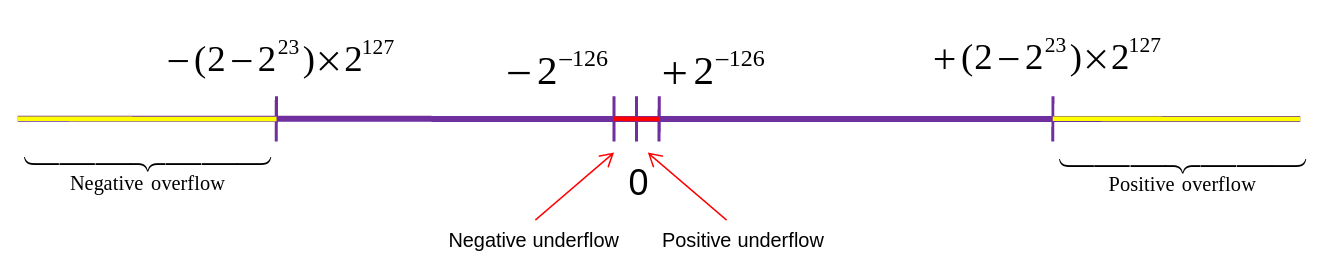
\includegraphics[width=\textwidth]{images/fp-range}
  \caption{\label{fig:fp-range} The range of single precision floating
  point numbers.}
\end{figure}

Sixty-four bit floating point numbers have one sign bit, $11$ exponent
bits and $52$ mantissa bits. This means their bias will be $2^{11} =
2048$ and the range will be $2 - 2^{52} \times 2^{2^{11}}$.

The standard also has special values built in:

\begin{description}
\item \textbf{Zero}: When the exponent is all zeros and the mantissa
equal to zero.
\item \textbf{Denormalised number}: If the exponent is all zero, but
the mantissa is non-zero, then the number is $-1^{sign} \times
0.m\times 2^{-126}$.
\item \textbf{Infinity}: Exponent is all 1's and mantissa is all
0's. The sign dictates between positive and negative infinity.
\item \textbf{NaN}: Not your grandma, this is when the value isn't a
  real number, such as when a division by zero occurs.The exponent is
  all 1's and the mantissa is non-zero.

NaN has two types; QNaN (quiet) and SNaN (signalling). SNan's has a
clear significant bit, and is used to signify an exception in
operations. QNaN is when the significant bit is set, and is assigned
when the result of a mathematical operation was not defined (but the
computation can still continue, with the NaN propagated).
\end{description}

% TODO: Special operations (slide 11)

\subsubsection{Quantifying error in floating point numbers}
% Example exam q:
% Given a decimal number x, convert it to normal form and then into binary
% with specific values for e, m and b. Then trunctuate/round it and estimate
% the error

When a real number is converted to floating point number, it may lose precision.
If the real number if $x$ and the floating point representation is
$\bar{x}$, then the error is:

\[
  e = \bar{x} - x
\]

You can find how many significant digits a floating point number approximates a
real number to by doing:

\[
  |\bar{x} - x| = b^{-\text{significant digits}}
\]

For example, if $x = 25.245$ and $\bar{x} = 25.255$ then $e = 25.255 -
25.245 = 10^{-4}$. We denote $\delta_x$ as the absolute error bound of
the floating point representation; $\bar{x} - \delta_x \leq
x \leq \bar{x} + \delta_x$.

However, the absolute error $e$ does not give us a very good description of the
accuracy (if the error is $10^{-6}$ but the value is $10^{-7}$ then we're very,
very inaccurate)! To rectify this, we have relative error:

\[
  r = \frac{e}{x} = \frac{\bar{x} - x}{x}
\]

Then we can define the relative error to be:

\[
  \epsilon_x = \frac{\delta_x}{|x|} \approx \frac{\delta_x}{|\bar{x}|}
\]

When we're getting the floating point number from the real number, we
can truncate the (possibly infinite) digits so that it fits in the
mantissa. Simply chopping the number so it fits in $m$ bits is
called \textbf{simple truncation}. Simple truncation introduces an
absolute error of $|e| = |\bar{x} - x| \leq b^{e-m}$

If we round numbers instead of using simple truncation, then we can reduce the
error. We need some rules though:

\begin{itemize}
\item If the part of the mantissa to be chopped of is less than $0.5$, use simple truncation.
\item If it's greater, then increment the mantissa, and then truncate.
\item If it's equal to $0.5$, then we can do either (though IEEE says to round up).
\end{itemize}

The easiest way to implement this on a computer is to do $x = x
+ \frac{b^{e-n}}{2}$, which always rounds up in the third case above.

Now the absolute and relative errors are:

\[
\begin{split}
  |e| &\leq \frac{b^{e-n}}{2}\\
  |r| &= \frac{|e|}{|x|} = \frac{0.5 \times b^{e-n}}{|m|\times b}\\
      &= \frac{1}{2 \times m \times b^n}
\end{split}
\]

\subsubsection{Types of error}

There are three types of errors that computers can make:

\begin{itemize}
  \item \textbf{Essential} errors are ones that cannot be avoided (e.g. from erroneous
  input).
  \item \textbf{Rounding} errors are when we have to approximate real numbers with
  floating point ones (as we saw above). This error can be measured and controlled.
  \item \textbf{Methodology} errors come into play when replacing one problem by another
  similar, easier but less accurate problem is done. The solution is close, but
  not exact.
\end{itemize}

Unfortunately, errors can propagate through a computation. We must know the
errors introduced by every operation a computer performs on floating point
numbers. If we know $e_x = \bar{x} - x$ and $e_y = \bar{y} - y$, what is $e_{x
\cdot y}$?

The error introduced by addition, subtraction, multiplication and division is:

\begin{description}
  \item Addition:
  \[
    \bar{x} + \bar{y} = (x + e_x) + (y + e_y) = (e_x + e_y) + (x + y)
  \]
  \[
    e_{x+y} = e_x + e_y
  \]
  \item Subtraction (similar to addition):
  \[
    e_{x-y} = e_x - e_y
  \]
  \item Multiplication:
  \[
    \bar{x} \times \bar{y} = (x + e_x) \times (y + e_y) =
      xy + xe_y + ye_x + e_xe_y
  \]
  However since $e_xe_y$ is small:
  \[
    e_{x \times y} \approx xe_y + ye_x
  \]
  \item Division (derivation is more complicated):
  \[
    e_\frac{x}{y} \approx \frac{1}{y}e_x - \frac{x}{y^2}e_y
  \]
\end{description}

Relative error can also be calculated:

\begin{description}
  \item Addition:
    \[
      r_{x+y} = \frac{e_{x+y}}{x + y} = \frac{x}{x + y}r_x + \frac{y}{x + y}r_y
    \]
  \item Subtraction:
    \[
      r_{x-y} = \frac{e_{x-y}}{x - y} = \frac{x}{x - y}r_x + \frac{y}{x - y}r_y
    \]
  \item Multiplication:
    \[
      r_{x \times y} = \frac{e_{x \times y}}{x \times y} \approx r_x + r_y
    \]
  \item Division:
    \[
      r_{x / y} = \frac{e_{x / y}}{x / y} \approx r_x - r_y
    \]
\end{description}

In general, $\bar{x} \circ \bar{y} = (x \circ y)(1 + r_{x \circ y})$.

\subsubsection{Error Propagation}

\marginpar{Remember, error propagation is not associative. The error from a
multiplication and then an add is probably not the same as doing the add then
the multiplication.}

While it is useful to know the error of one operation, we also need to be able
to work out the error of consecutive operations. That is to say given $e_x =
\bar{x} - x$ and  $e_y = \bar{y} - y$, determine $e_{x \bar{\circ} y}$.
\[
  \begin{split}
  \bar{x} &= FP(\bar{x_1} \circ \bar{x_2})\\
          &= \bar{x_1} \bar{\circ} \bar{x_2}\\
          &= (\bar{x_1} \circ \bar{x_2})(1 + u)\\
  \end{split}
\]

Where $|u| \leq 0.5 \times b^{-n + 1}$ is the machine relative
round-off error.

The total error and total relative error is given by:

\[
\begin{split}
  e^t_z &= \bar{z} - z = z(r_{x \circ y} + u + r_{x \circ y} \cdot
  u) \approx z(r_{x \circ y} + u)\\
  r^t_z &= \frac{e^t_z}{x} = r_{x \circ y} + u = a_xr_x + a_yr_y + u
\end{split}
\]

Where $a_x$ and $a_y$ is the error introduced by the $\circ$ operation.

Lets put all that into an example. Given the numbers $x,y$ and $x$ with their
relative round off errors $r_x, r_y$ and $r_z$, determine the relative error in
$u = (x + y)z$:

\[
  r^t_{x + y} = \frac{x}{x + y}r_x + \frac{y}{x + y}r_y + r_+
\]

\[
  r^t_{u} = \left(\frac{x}{x + y}r_x + \frac{y}{x + y}r_y + r_+\right) + r_z + r_*
\]

% TODO: How to do the next bit on slide 23

\subsection{Finding the number of significant digits}

We want to find an integer that represents how many digits in our number are
non-nonsense (i.e. how many significant digits we have). The number of
significant digits in the floating point number $\bar{x}$ where its real
equivalent is $x$ is given by:

\marginpar{$Z(x)$ gives the integer closest to the real number $x$.}

\[
  l = Z(log_b\frac{|x|}{|\bar{x} - x|})
\]

Therefore, the relative error is:

\[
  r_x \approx b^{-l}
\]

If we have a computation that takes $m$ real numbers as arguments and outputs a
real number, if the arguments are floating point numbers with $l_i$ significant
digits then we can estimate:

\[
  |e| \approx |\sum^m_{i=1} x_i\frac{\delta f}{\delta x_i}b^{-l_i}|
\]

Also:

\[
  |\sum^m_{i=1} x_i\frac{\delta f}{\delta x_i}b^{-l_i}|
    \leq b^{-l_{min}}|\sum^m_{i=1} x_i\frac{\delta f}{\delta x_i}|
\]

The number of significant digits in the answer is:

\[
  l = l_{min} - \delta
\]

Where $\delta$ is the loss of significant digits:

\[
  \delta = Z(log_b(
    \frac{
      \sum^m_{i=1}|x_i\frac{\delta f}{\delta x_i}|
    }{
      |f(x_1, \dots, x_m)|
    }
  )
\]

If we try and subtract numbers that are close in magnitude, then we will lose
lots of significant digits. If we do $\sqrt{2.01} - \sqrt{2}$ (where both
numbers are known to 9 significant digits), then we get:

\[
  \delta = Z(log_10(
    \frac{
      |\sqrt{2.01}| + |\sqrt{2}|
    }{
      |\sqrt{2.01} - \sqrt{2}|
    })) = 3
\]

Our answer would be to six significant figures. In order to get all of the
significant figures, we need to use a different method:

\[
  \begin{split}
    z &= \sqrt{2.01} - \sqrt{2}\\
      &= (\sqrt{2.01} - \sqrt{2})\frac{\sqrt{2.01}
         + \sqrt{2}}{\sqrt{2.01} + \sqrt{2}}\\
      &= \frac{\sqrt{2.01}^2 - \sqrt{2}^2}{\sqrt{2.01} + \sqrt{2}}\\
      &= \frac{0.01}{\sqrt{2.01} + \sqrt{2}}
  \end{split}
\]

\marginpar{Revision break? Read this:
\href{https://randomascii.wordpress.com/2014/01/27/theres-only-four-billion-floatsso-test-them-all/}{https://randomascii.wordpress.com
/2014/01/27/theres-only-four
-billion-floatsso-test-them-all/}}

\subsubsection{Accurately computing sample variance}

Computing the sample variance of a set of numbers is done by the formula:

\[
  s^2_n = \frac{1}{n - 1}\sum^n_{i=1}(x_i - \hat{x})^2
\]

Where $\hat{x} = \frac{1}{n}\sum^n_{i=1}x_i$ is the mean of the values.

In order to compute the variance, we would need to calculate the mean first,
then calculate the variance, which requires two for loops. However, a
numerically equivalent formula exists for doing the same thing:

\[
  s^2_n = \frac{1}{n-1}(\sum^n_{i=1}x_i^2 - \frac{1}{n}(\sum^n_{i=1}x_i)^2)
\]

If we use the following data:

\begin{center}
  \begin{tabular}{>{$}c<{$}|>{$}c<{$}}
    \text{Value} & \text{Floating point representation}\\ \hline
    100 & 0.1000\times10^3\\
    101 & 0.1010\times10^3\\
    102 & 0.1020\times10^3
  \end{tabular}
\end{center}

If we use formula one for the variance with these input numbers, then we get an
answer of $1$, if we use formula two, then we get the answer to be $-1.667$

% TODO: Why???

\subsubsection{Overflow and underflow}

We must be aware of overflow and underflow in our operations. For example, if we
were calculating the length of the hypotenuse of a triangle
($\sqrt{\text{opposite}^2 + \text{adjacent}^2}$), then we could have an overflow
if $x = y = 10^{200}$, since the range representable by a single precision float
is $10^{\pm308}$.

This can be remedied by using a different formula:

\begin{center}
  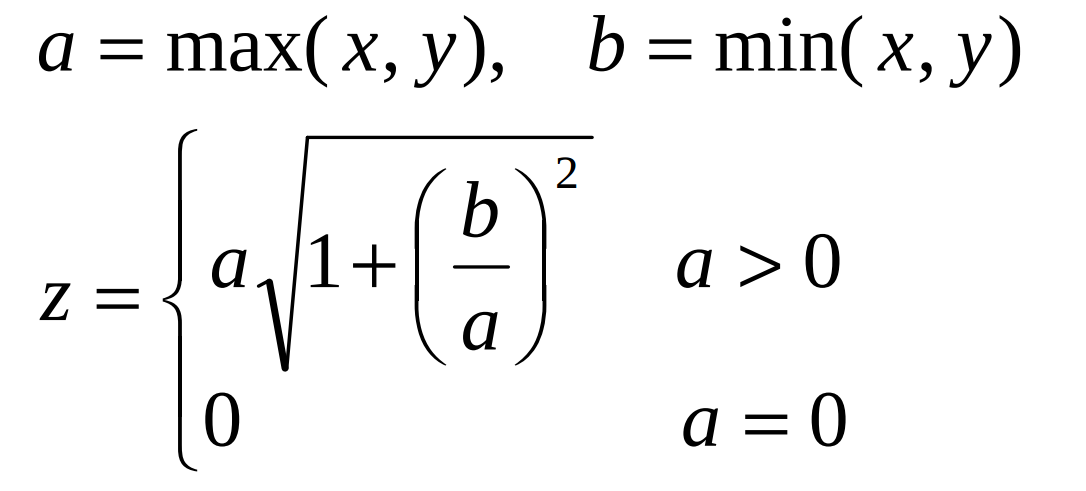
\includegraphics[width=0.3\textwidth]{images/safe-pythag}
\end{center}

\subsection{Condition of a problem}

The condition of a problem is how sensitive it is to changes in the data. A
problem is ill-conditioned if a small change in the data results in a large
change in the solution. This is concerned with the problem, not the method used
to solve it.

Consider the equation $x^3 - 21 x^2 + 120x - 100 = 0$; the solutions are $x =
\{1, 10\}$. However, if we change the value of $x^3$ to $0.99$ or $1.01$, then
the roots become $x = \{1, 11.17, 9.041\}$ and $x = \{1, 9.896 \pm 1.044\}$
respectively.

We can work out the sensitivity by using partial differentiation, if the
perturbed function if $\bar{f}(x) = f(x) + \epsilon g(x)$, where $g(x)$ is the
change applied to $f(x)$, then:

\[
  |\delta| \approx |\frac{\epsilon g(x)}{f'(x)}|~\text{(single root)}
\]

\[
  |\delta| \approx |\sqrt{-\frac{2\epsilon g(x)}{f''(x)}}|~\text{(double root)}
\]

In the above example, $g(x) = x^3, \epsilon = -0.01, f'(x) = 3x^2 - 42x + 120$:

\[
  |\delta| \approx |\frac{-0.01 \times 1^3}{81}| \approx 0.0001
\]

For the double root, $f''(x) = 6x - 42$

\[
  |\delta| \approx |\sqrt{-\frac{2 \times -0.01 \times 1000}{18}}| \approx 1.054
\]

So the double root is vastly affected, but the single root isn't.

\subsection{Stability}

The stability of a method is how sensitive it is to rounding errors. A method
that guarantees as accurate solution as the input data allows is said to be
stable, otherwise it's unstable. Condition is about the sensitivity of the
problem, but stability is about the sensitivity of the method.

Given the quadratic equation $1.6x^2 - 100.1x + 1.251 = 0$, the solution can be
found using the standard formula (in floating point) ($x = \frac{-b \pm\sqrt{b^2
- 4ac}}{2a}$), which gives $x = \{62.53, 0.03125\}$.

If we only compute the first root to be $x_1 = 62.53$, but use $x = c/ax_1$ for
the second, then we get the second root to be $0.01251$. The correct solutions
are $x = \{62.53, 0.0125\}$.

The problem was that $y_1 = -b = 100.1$, and  $y_2 = \sqrt{b^2 - 4ac} = 100.06$.
Since if we do subtraction with very close numbers, the error is high. If we
calculate $\delta$ for this then we get:

\[
  \delta = X(log_10\frac{|y_1| + |y_2|}{|y_1 - y_2|}) = 4
\]

Meaning all of our digits were rubbish!

%TODO: Page 41 onwards for an example
